\chapter{Projekt}
\label{cha:projekt}

W tym rozdziale opisana jest realizacja praktyczna projektu. Najpierw omówione zostaną wymagania stawiane całej aplikacji i podstawowe
założenia związane z jej implementacją. Nastepnie przybliżone zostaną jej poszczególne komponenty.

\section{Wymogi i założenia}
\label{sec:wymogi}

\subsection{Budowa}
\label{subs:budowaAplikacji}

Podstawowym celem projektu jest implementacja oprogramowania pobierającego z podzbioru stron opublikowanych w Internecie dokumenty i przedstawiającego
je w postaci omówionych w Rozdziale \ref{cha:budowaGrafu} asocjacyjnych grafów AGDS. Jest to zadanie wieloetapowe, wymagające następujących komponentów:
\begin{enumerate}
\item Robota dostarczającego dane z sieci. Komponent musi mieć możliwość asynchronicznego pobierania stron WWW, udostępniać API do estrakcji adresów URL z ostatnio
ściągniętych stron spełniających podane warunki oraz implementować \emph{Robots Exclusion Protocol}.
\item Komponentu współpracującego z wyżej opisanym modułem, zapweniającego interfejs umożliwiający zapisywanie danych do zewnętrznej bazy. Umożliwiającego
zapisaywanie kolejnych wersji stron WWW, opisanych \emph{timestampem}.
\item Modułu przetwarzającego wybrane strony WWW przechowywane w zewnętrznej bazie. Powinien on być dawać możliwość parsowania strony HTML i operowania na drzewie DOM.
Powinien mieć możliwość zapisu informacji w formacie JSON, przy zachowaniu budowy umożliwiającej proste rozszerzanie funkcjonalności poprzez dodawanie odpowiednich klas do projektu.
\item Prostego klienta kolejki RabbitMQ, wykonującego RPC z przetworzonymi wcześniej danymi, jako argumentem.
\item Serwera odbierającego wywołania przez kolejkę RabbiMQ, rozpoczynającego konwersję danych do formatu AGDS i zwracającego wynik na kolejkę.
\item Modułu przetwarzającego dane odebrane przez serwer, dzielącego wysyłane strony na sekwencje uczące, umożliwiającego w razie potrzeby proste rozszerzenie funkcjonalności.
\item Silnika asocjacyjnego współpracującego z warstwą zapewniajacą persystencję. Jego jedynym zadaniem jest budowa grafu AGDS zgodnie z założeniami opisanymi w Rozdziale
\ref{cha:budowaGrafu}.
\item Warstwy pośredniczącej pomiędzy aplikacją, a bazami danych. Powinna ona zapisywać logiczną strukutrę grafu w bazie grafowej, a dodatkowe informacje, takie jak
atrybuty poszczególnych węzłów(np. częstość występowania), czy krawędzi(np. waga) przechowywać wl ekkiej bazie klucz~-~wartość. Ważne jest ukreywanie szczegółów implementacyjnych,
zwłaszcza wynikających z używania wielu rodzajów baz danych.
\end{enumerate}

W związku ze skalą projektu i trudnym debugowanie komunikujących się ze sobą modułów, każdy komponent posiada testy jednostkowe.

\subsection{Podział aplikacji}

W celu lepszej organizacji kodu, jak i separacji odpowiedzialności poszczególnych elementów aplikacji, postanowiono wydzielić z niej dwa podstawowe moduły:
\begin{enumerate}
\item Składający się z komponentów 1. - 4. moduł odpowiedzialny za ściąganie i przechowywanie danych z sieci. Może on być tratkowany jako repozytorium
nieprzetworzonych danych, które można używać wielokrotnie dla różnych eksperymentów.
\item Składający się z komponentów 5. - 8. wyspecjalizowany moduł odpowiedzialny za budowę i przechowywanie struktury AGDS. Jest on niezależny od konkretnego źródła
danych, wymaga jedynie ich określonego formatu.
\end{enumerate}

Oba moduły są połączone kolejką z zaimplementowanym protokołem RPC.

\begin{figure}[!h]
    \centering
    \label{graph:aplikacja}
    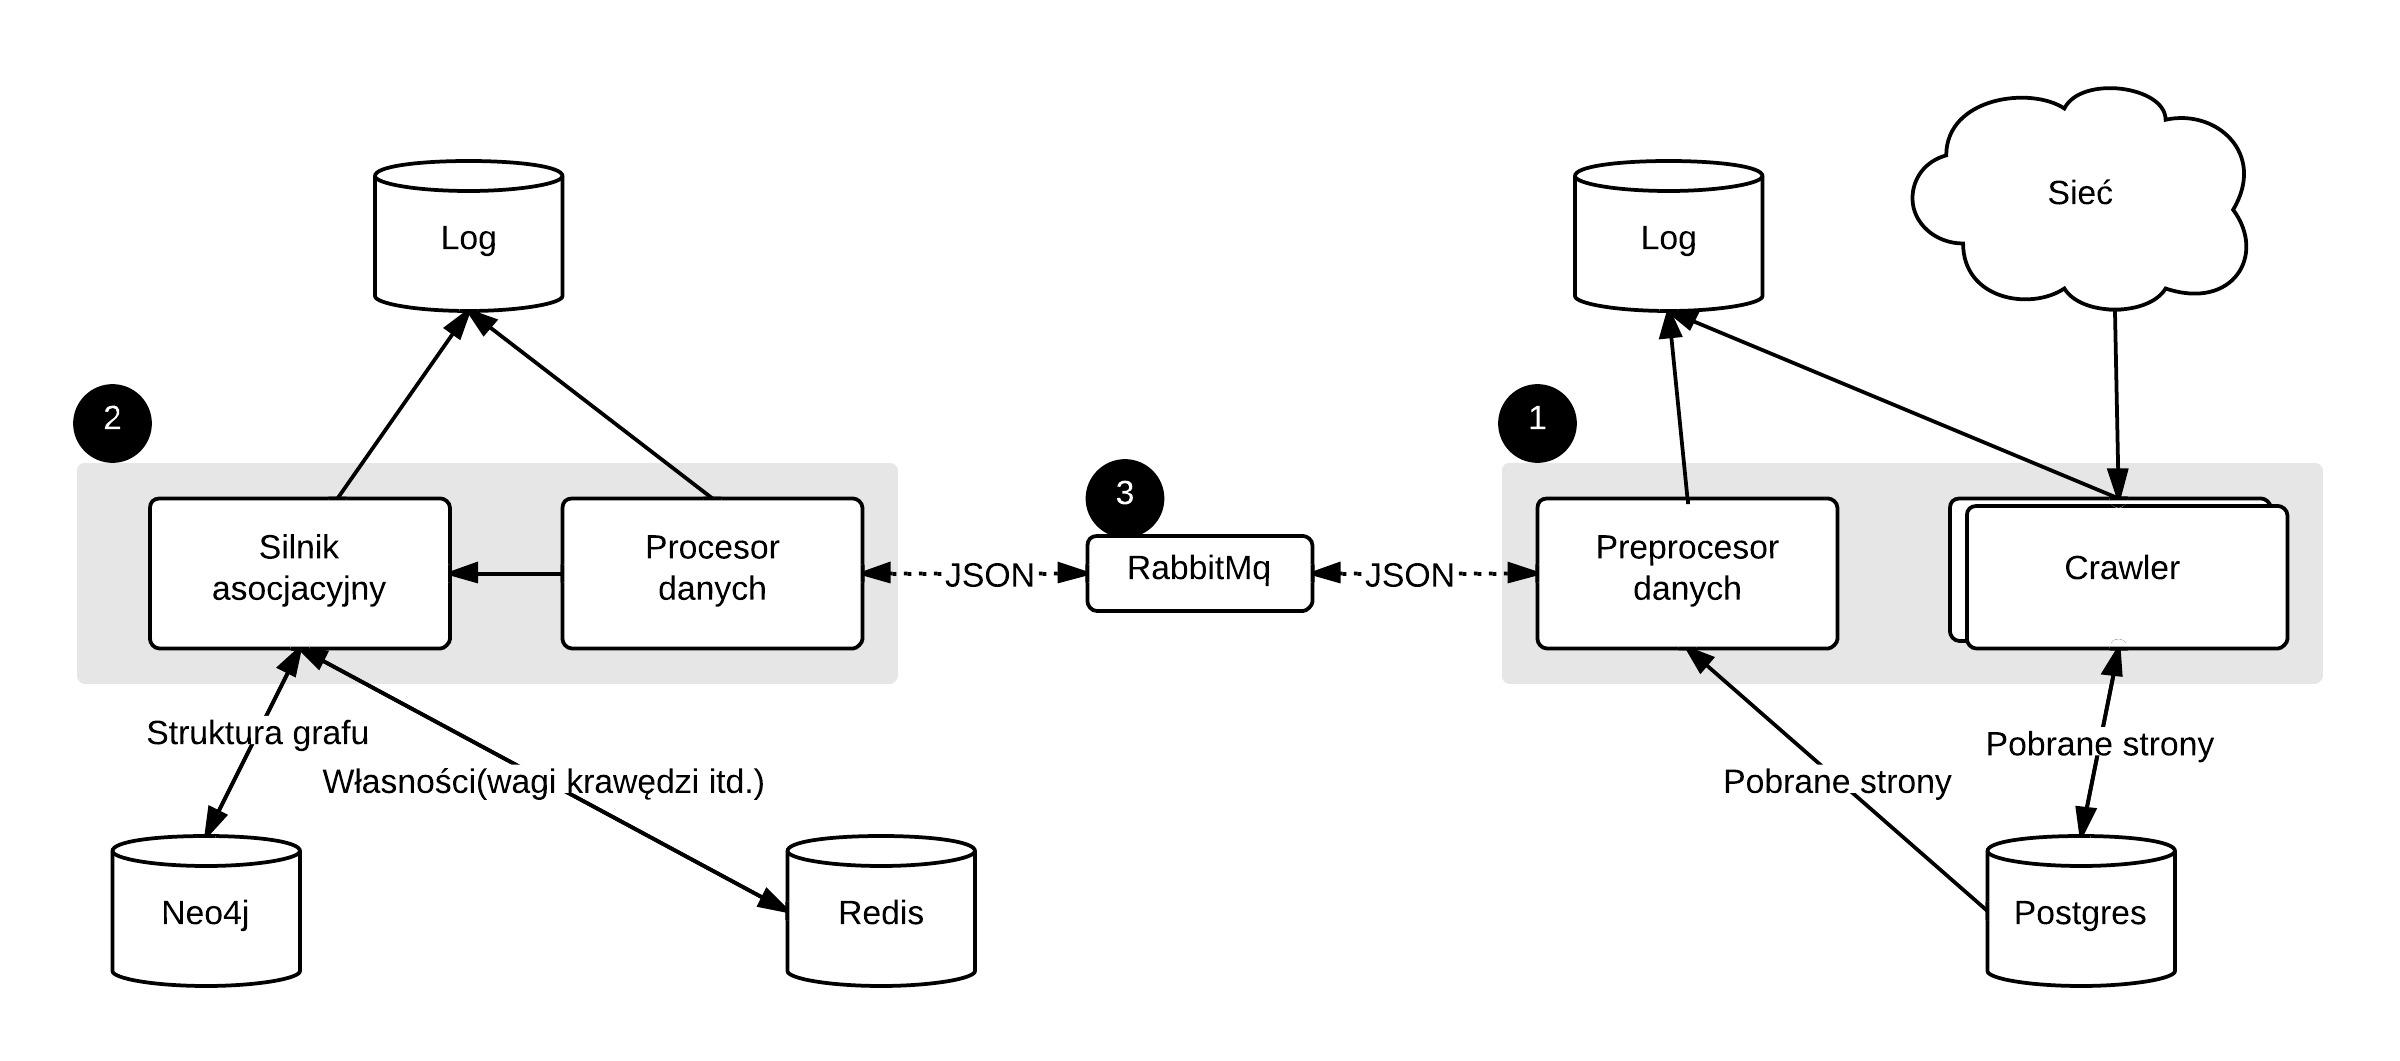
\includegraphics[scale=0.2]{aplikacja}
    \caption{Schemat architektury aplikacji. 1. - część pobierająca dane, 2. - część konstruująca graf 3. - kolejka}
\end{figure}

\subsection{Wejście/wyjście}
\label{subsec:weWy}

Aplikacja nie posiada interfejsu graficznego. Poszczególne komponenty są wzbudzane z poziomu \emph{shella}, konfiguracja odbywa się poprzez edycję wydzielonych plików konfiguracyjnych, 
opcje podawane przy wykonywaniu skryptów lub zmienne środowiskowe. Celem tej części projektu nie jest serwowanie użytkownikowi informacji, a przedstawianie danych w pewny określonym
formacie, stąd takie ograniczone spektrum możliwości interakcji z aplikacją. Konkretne skrypty uruchamiające aplikacje, opcje ich wywoływania i struktura plików konfiguracyjnych opisana 
jest w dalszej części pracy.

\section{Opis komponentów 1. - 4.}

Na rysunku \ref{graph:mri} przedstawiony jest detaliczny schemat pierwszych czterech komponentów głównej aplikacji. W istocie tworzą one autonomiczną subaplikację, powiązaną z resztą
komponentów jedynie poprzez kolejkę.. 

\begin{figure}[!h]
    \centering
    \label{graph:mri}
    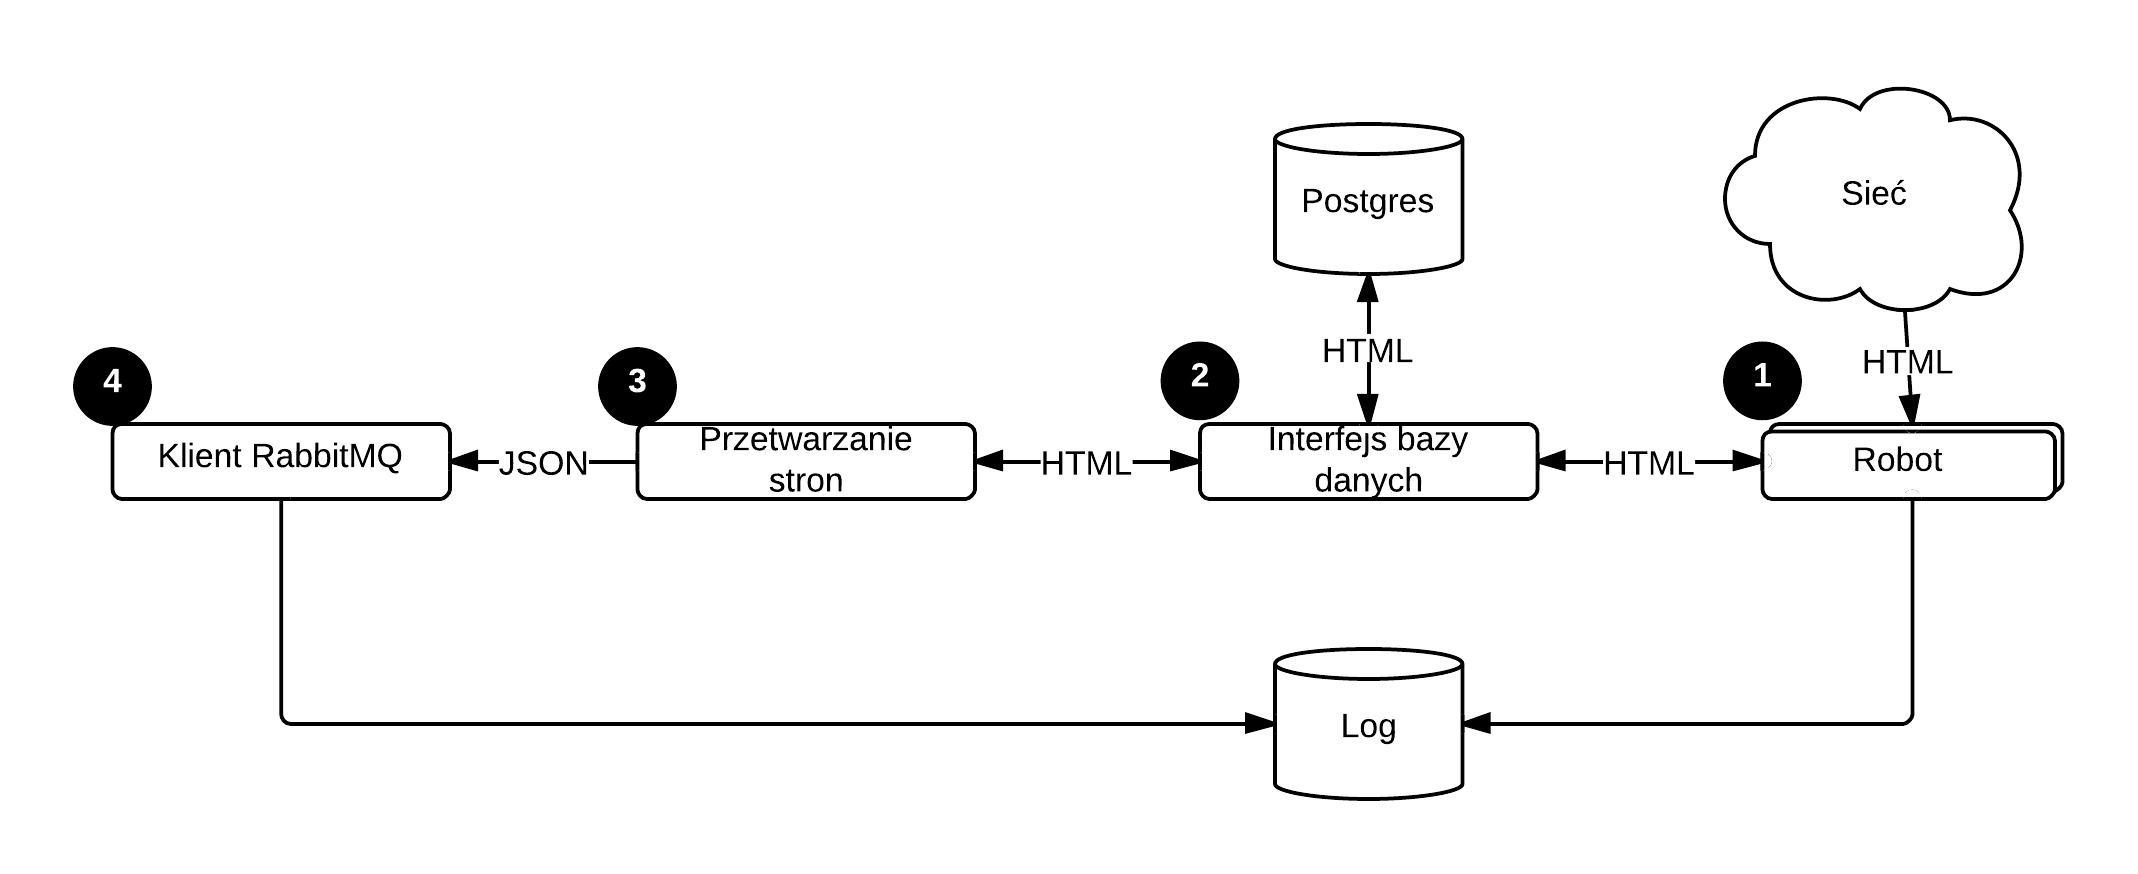
\includegraphics[scale=0.22]{mri}
    \caption{Detaliczny schemat komponentów 1. - 4. Podpisy na strzałkach odnoszą się do formatu, w jakim przedstawiane są strony internetowe na każdym z prezentowanych etapów. }
\end{figure}

\subsection{Struktura przechowywanych informacji}
\label{subs:struktMri}

\begin{figure}[!h]
    \centering
    \label{graph:mri_schema}
    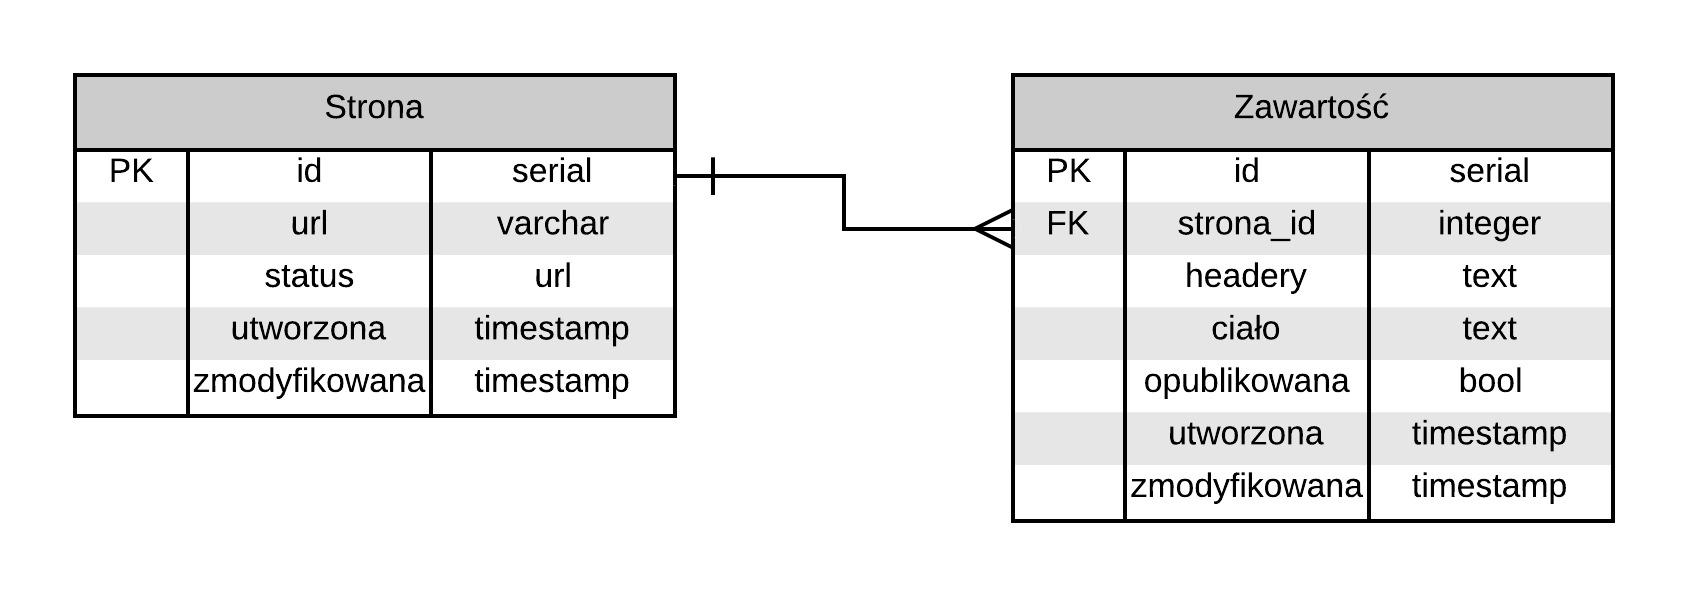
\includegraphics[width=\textwidth]{mri_schema}
    \caption{Schema przechowująca informacje pobrane z sieci.}
\end{figure}

Struktura bazy umożliwia przechowywanie unikalnych adresów URL w relacji \texttt{Strona} i zapisywanie historii kolejnych odwiedzin w osobnej tabeli \texttt{Zawartość}. Dzięki
temu otrzymuje się prosty sposób na archiwizację nieaktualnych rekordów, przy braku konieczności modyfikacji bazy. Następnie takie rekordy mogłyby być cyklicznie przenoszone 
np.~do hurtowni danych, w celu późniejszej analizy. Dodatkowego wyjaśnienia wymagają dwa pola: pole \texttt{strona.status} przyjmujące wartości ze zbioru: 
$\{oczekuje, pobierana, sukces, blad\}$, odpowiadające cyklowi pobierania i przetwarzania informacji. Wartość $pobierana$ ma na celu niedopuszczenie do pobierania tej samej
strony przez dwa procesy robota. Drugie to pole \texttt{wartość.opublikowana} odnosi się do faktu wysłania danej zawartości do kolejki. Jeżeli to nastąpiło i komponent nie otrzymał
w odpowiedzi zwrotnej komunikatu o błedzie, wartością tego pola wynosić będzie TRUE, w przeciwnym razie FALSE.

\subsection{Przepływ danych}
\label{subs:mriPrzepDanych}

Aplikacja posiada dwie niezależne ścieżki przepływu i przetwarzania danych:
\begin{enumerate}
\item Ścieżka związana z pobieraniem danych z sieci.
\item Ścieżka przetwarzania ściągniętych danych i publikacja ich za pomocą kolejki.
\end{enumerate}

Pierwsza ścieżka przedstawiona jest na rysunku \ref{graph:mri_przeplyw_1}. Uruchamiany jest robot, który po odczytaniu konfiguracji i nawiązaniu połączenia z bazą danych zaczyna pobierać
automatycznie dane z sieci.  Liczba procesów wykonujących to zadanie nie ma narzuconego z góry ograniczenia, dane między procesami są synchronizowane na poziomie dostępu do bazy danych.
Jak można zauważyć przedstawiony schemat nie różni się od podstawowej implementacji crawlera przedstaionej w rozdziale \ref{cha:pozyskiwanieTresci}.

Rolę listy adresów URL przejęła baza danych. Jest to może rozwiązanie nieefektywne, ale proste w implementacji i wystarczające dla niniejszego projektu.
W razie konieczności przyspieszenia działania robota można zastosować lekką bazę NoSQL, jak Redis, czy rozwiązanie cache'ujące, takie jak Memcached.
W celu oszczędzenia czasu, nie zawsze następuje ekstrakcja adresów URL i dodawanie ich do bazy. Dzieje się to jedynie wtedy, gdy liczba adresów oczekujących
jest mniejsza, niż czterokrotność liczby adresów odwiedzonych. 

Druga ścieżka przepływu danych ma prostszy przebieg, dlatego ograniczone się jedynie do wypisania jej poszczególnych kroków.
\begin{enumerate}
\item Pobranie nieopublikowanego(flaga \texttt{opublikowana} ma wartość FALSE) rekordu z tabel \texttt{Zawartość}.
\item Parsowanie ciała strony za pomocą biblioteki Nokogiri.
\item Pobranie z drzewa DOM interesujących elementów, np. całej zawartości umieszczonej między znacznikami HTML <p>\dots</p> i podzielenie jej na dwie grupy: pierwszą, która
obowiązkowo musi zostać użyta do budowy grafu AGDS(np. tekst umieszczony w nagłówkach) i drugą, która zawiera przydatne, ale mniej wartościowe informacje - np. tekst z ciała artykułu.
\item Zapis tak przygotowanego tekstu  do dwóch tablic, kolejno dla pierwszej i drugiej grupy.
\item Dodanie informacji o adresie URL przetwarzanej strony, zakodowanie jako JSON i opublikowanie poprzez kolejkę.
\end{enumerate}

\newpage

\begin{figure}[!h]
    \centering
    \label{graph:mri_przeplyw_1}
    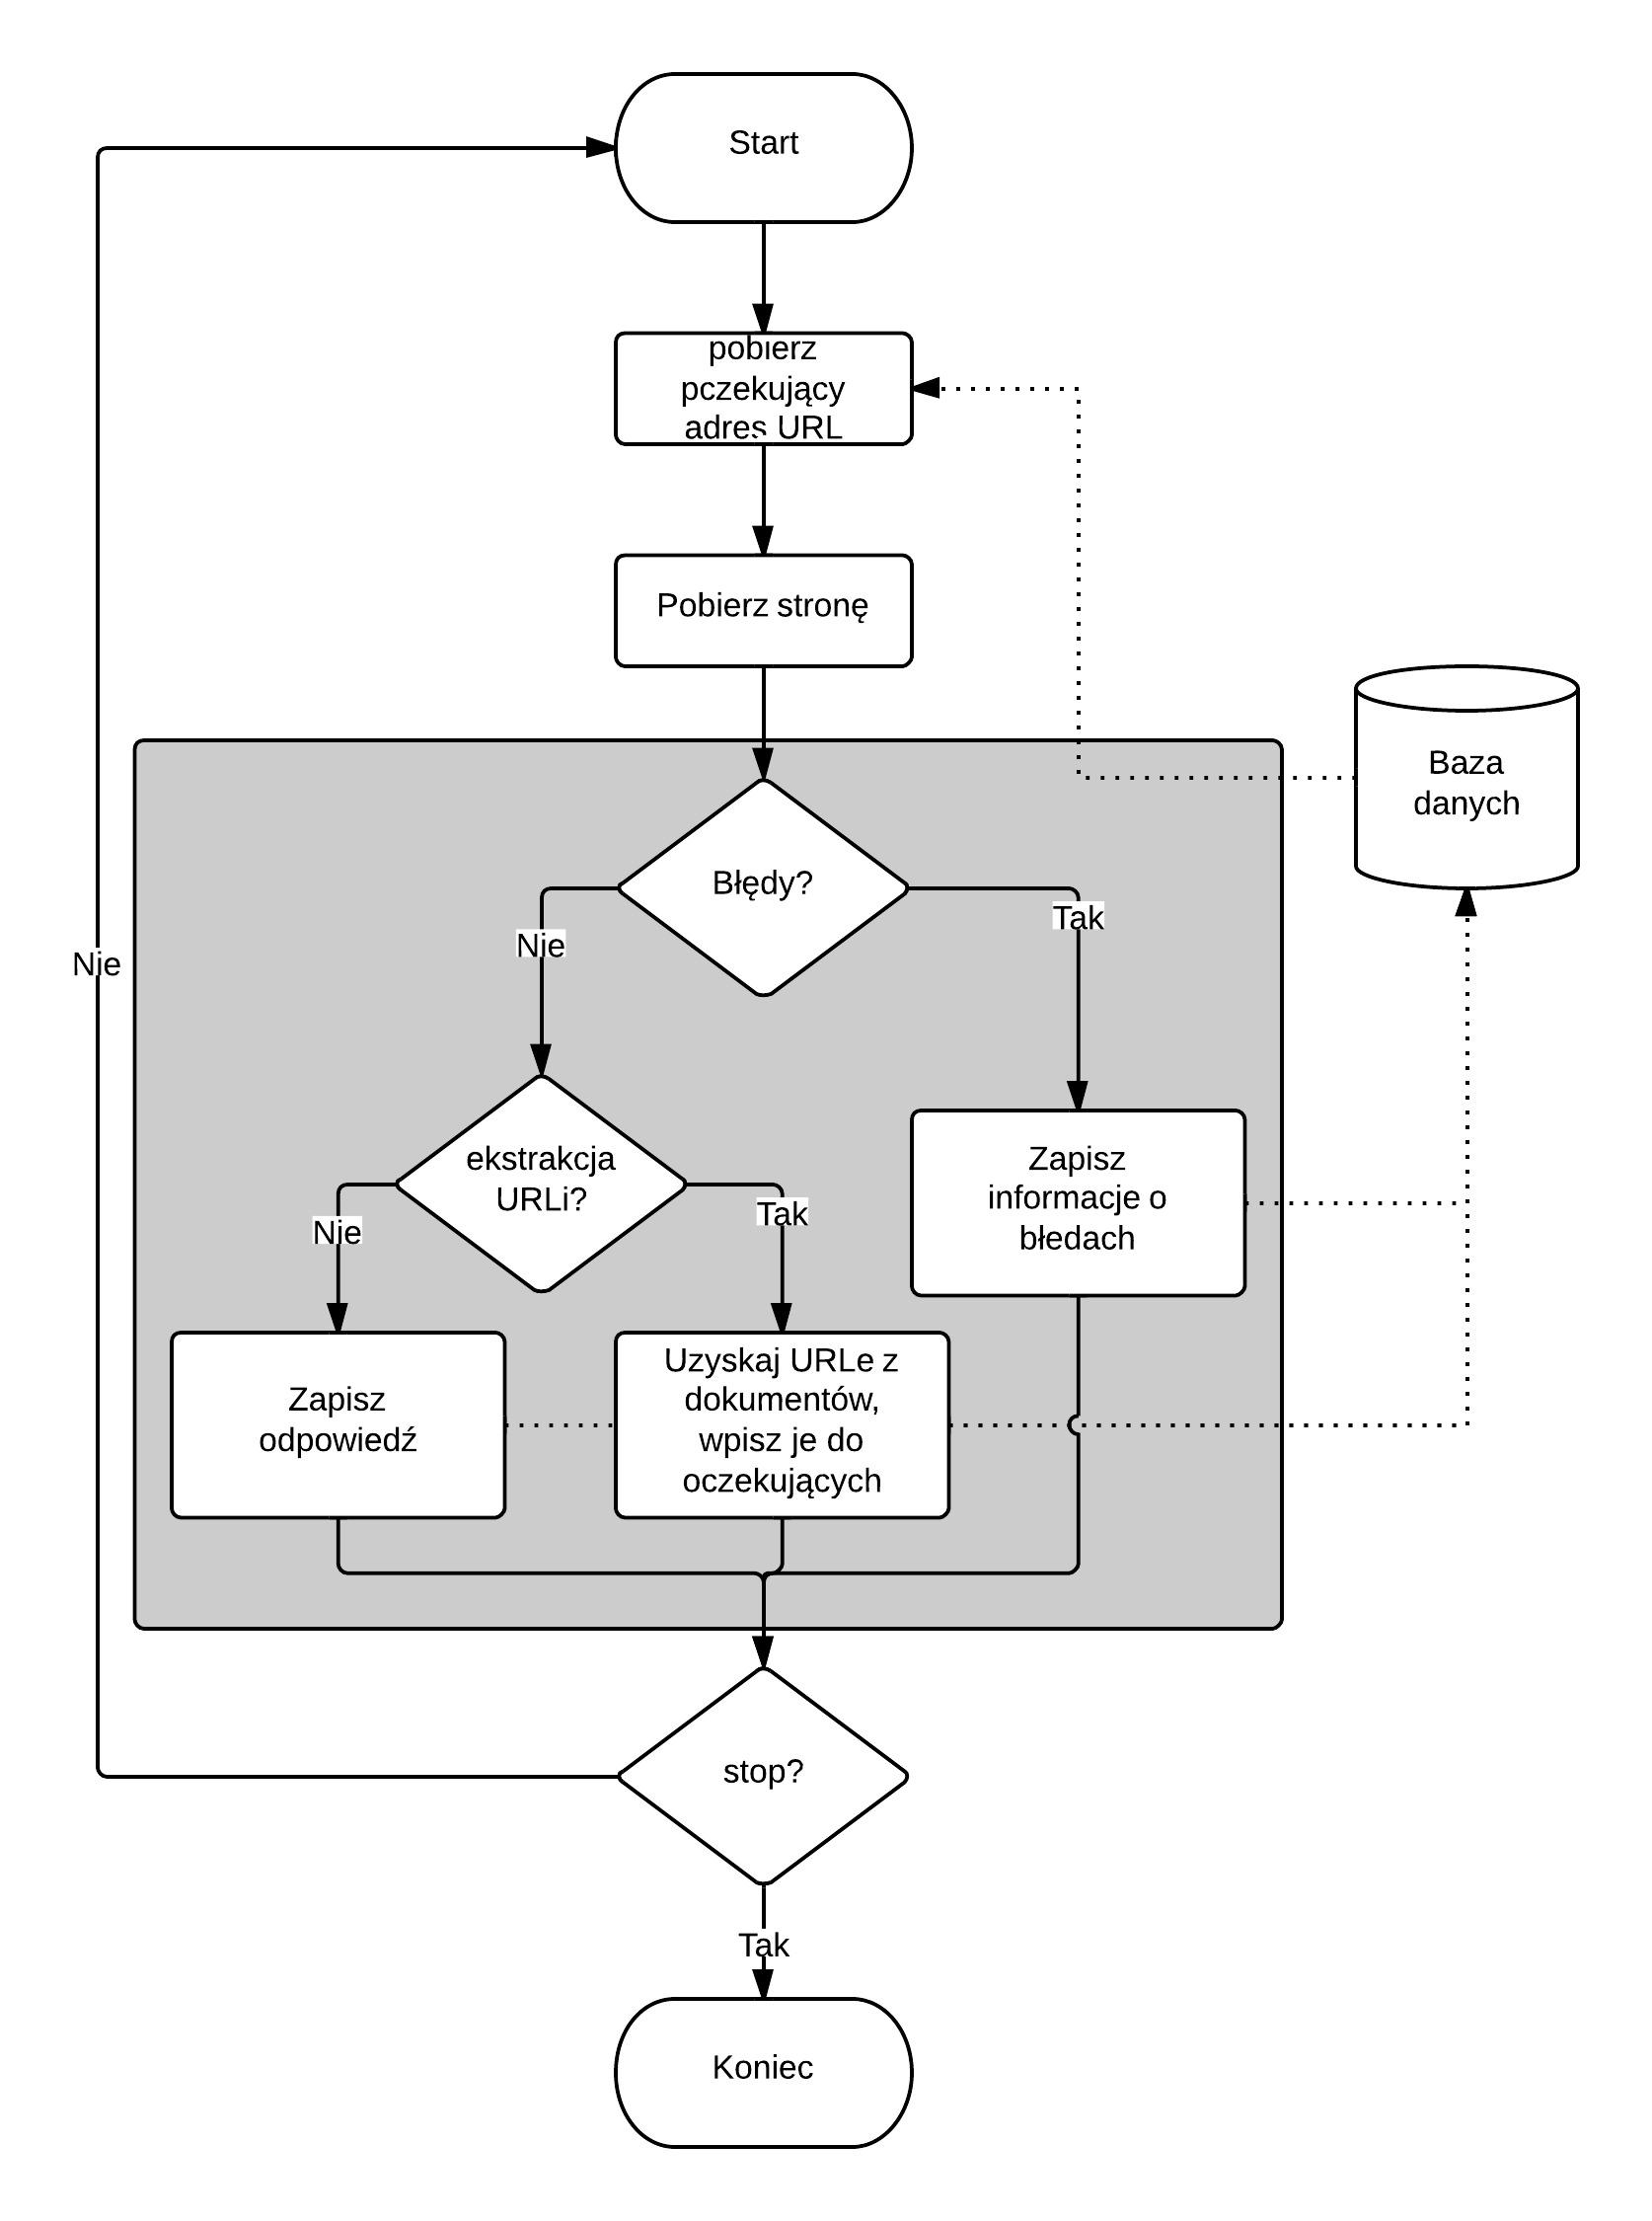
\includegraphics[width=\textwidth]{mri_przeplyw_1}
    \caption{Schemat pierwszej ścieżki przepływu. Dla przejrzystości nie uwzględniono asynchronicznego sposobu pobierania stron.}
\end{figure}


\section{Opis komponentów 5. - 8.}

Na rysunku \ref{graph:neo4j} przedstawiony jest detaliczny schemat reszty aplikacji. Jest to również kod pracujący autonomicznie, jedynym punktem wejścia
jest serwer nasłuchjący na kolejce.

\begin{figure}[!h]
    \centering
    \label{graph:neo4j}
    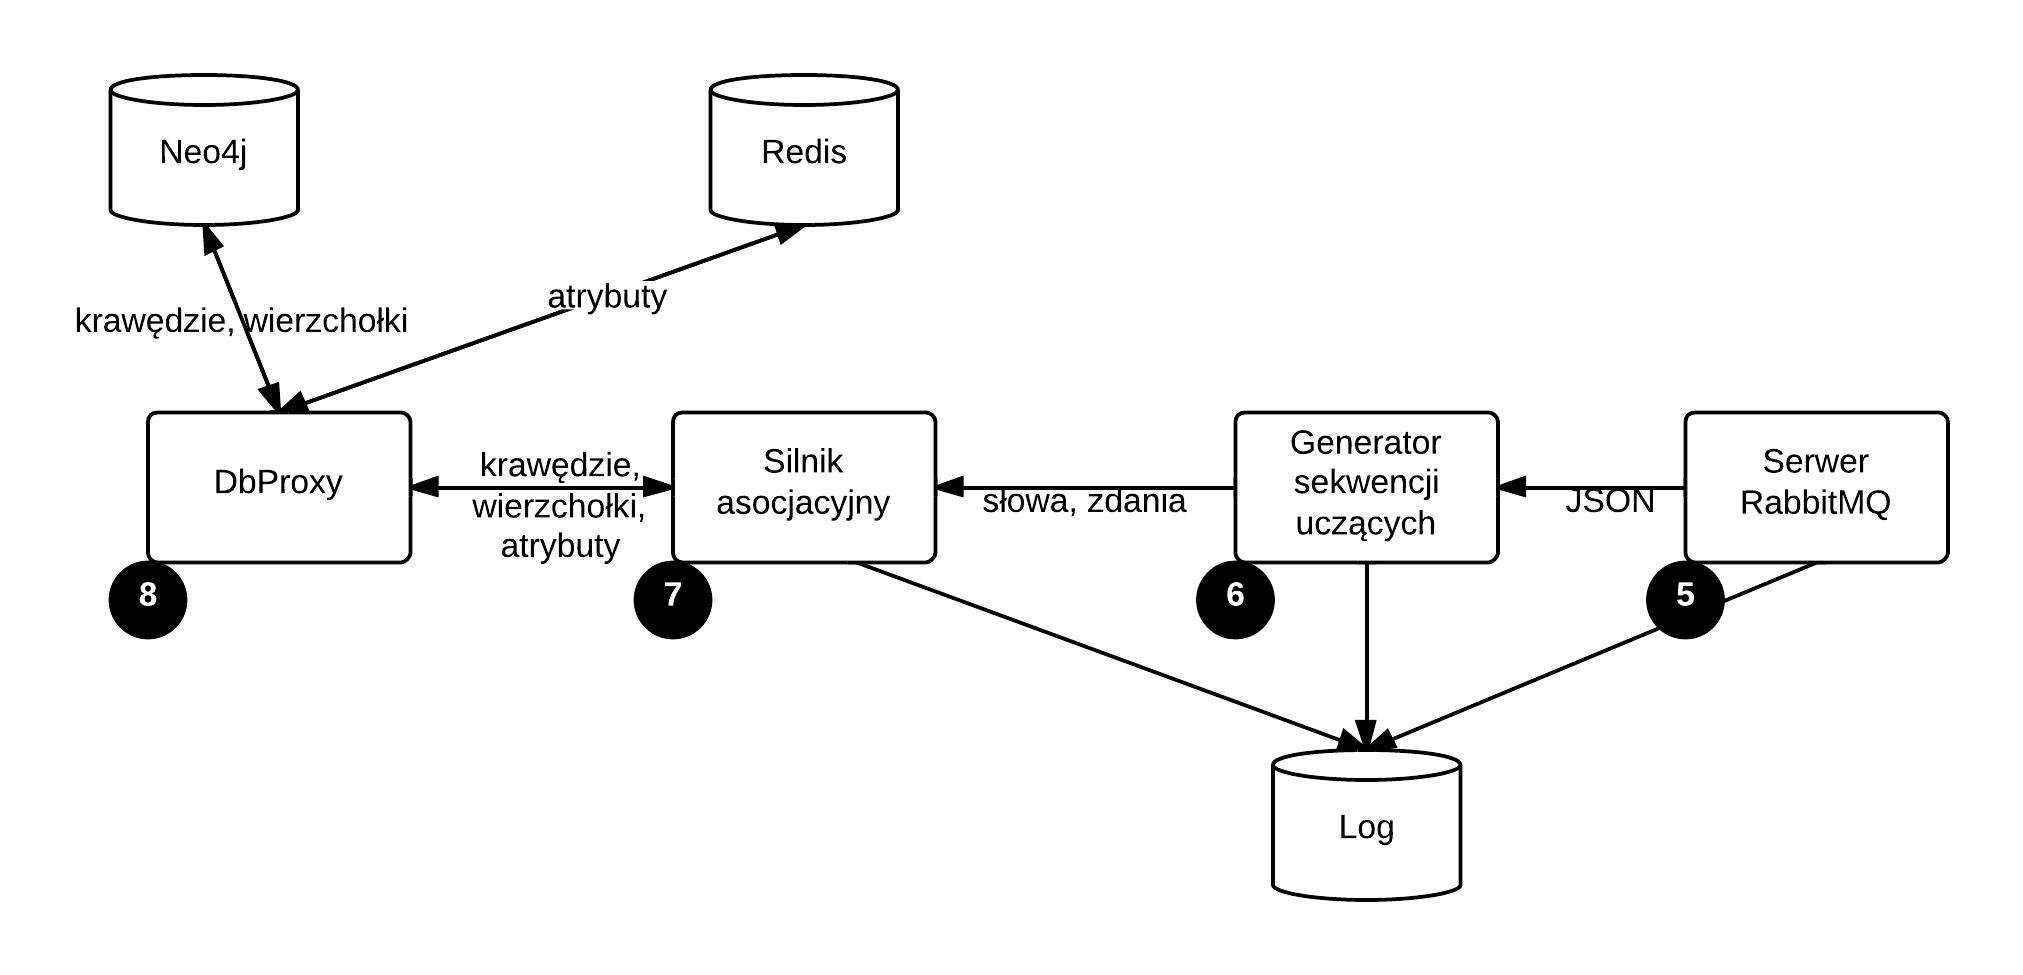
\includegraphics[scale=0.22]{neo4j}
    \caption{Detaliczny schemat komponentów 5. - 8. Podpisy na strzałkach odnoszą się do formy, jaką przyjmują przepływające przez aplikację dane.}
\end{figure}

\subsection{Struktura przechowywanych informacji}
\label{subs:struktNeo4j}

Jak wspomniano wcześniej, baza grafowa cechuje się większą elastycznością, niż tradycyjne bazy relacyjne. Nie używa ona schematów, użytkownicy mają dowolność w kształtowaniu 
grafu i wielopoziomowych relacji łączących jego elementy.

\subsection{Przepływ danych}
\label{subs:mriPrzepDanych}

Ten komponent posiada tylko jedną ścieżkę przepływu danych, wiązaną z tworzeniem struktury AGDS. Poniżej opisane są wszystkie przekształcenia, którym poddaje się dane
odbierane przez serwer.

\begin{enumerate}
\item Odebranie danych przez serwer w postaci tesktowej, konwersja formatu JSON na obiekty natywne
\item Usunięcie nieprzydatniych ciągów znaków, np. charakterystycznego dla Wikipedii ciągu ``[edit]'' traktowanego przez parser HTML jak tekst, a niewnoszącego nowych informacji.
\item Podział tekstu, używając wyrażeń regularnych, na zdania i słowa.
\item Usunięcie zbyt krótkich słów, podział zbyt długich naturalnych zdań na krótsze(wydzielenie kontekstu). 
\item Ujednolicenie kodowania(UTF-8), konwersja do małych liter.
\item (opcjonalny) Stemming poszczególnych słów.
\item Podanie tak utworzonej sekwencji uczącej na wejście silnika asocjacyjnego.
\item Zapis utworzonego grafu do baz danych.
\end{enumerate}

Serwer oczekuje danych w postaci:

\lstset{language =JavaScript}
\begin{lstlisting}
{ url: "http://www.example.com/", body: ["pierwsze zdanie", "drugie zdanie"] }
//lub
{ url: "http://www.example.com/", body: { obligatory: ["Naglowek 1", "Naglowek 2"], optional ["zdanie 1", "zdanie 2"] } }
\end{lstlisting}

